\documentclass[tikz,border=8pt]{standalone}
% Shared look for every TikZ diagram. Load with \input{../../tools/tikz-style.tex}
\usepackage[T1]{fontenc}
\usepackage{lmodern}
\renewcommand{\sfdefault}{lmr}  % diagrams use the same serif as the text
\usetikzlibrary{arrows.meta, positioning, shapes.geometric, calc, fit, backgrounds}
\definecolor{cblue}{HTML}{4C78A8}
\definecolor{corange}{HTML}{F58518}
\definecolor{cgreen}{HTML}{54A24B}
\definecolor{cred}{HTML}{E45756}
\definecolor{cpurple}{HTML}{B279A2}
\definecolor{cgrey}{HTML}{6B6B6B}
\tikzset{
  every picture/.style={font=\sffamily, line width=1.2pt},
  box/.style={draw=#1, fill=#1!12, rounded corners=4pt, align=center, inner sep=7pt, minimum height=1.1cm},
  box/.default=cgrey,
  arrow/.style={-{Stealth[length=3mm]}, draw=cgrey, line width=1.4pt},
  title/.style={font=\sffamily\bfseries\Large},
  note/.style={font=\sffamily\small, text=cgrey, align=center},
}
\AtBeginDocument{\hyphenpenalty=10000 \exhyphenpenalty=10000}

\begin{document}
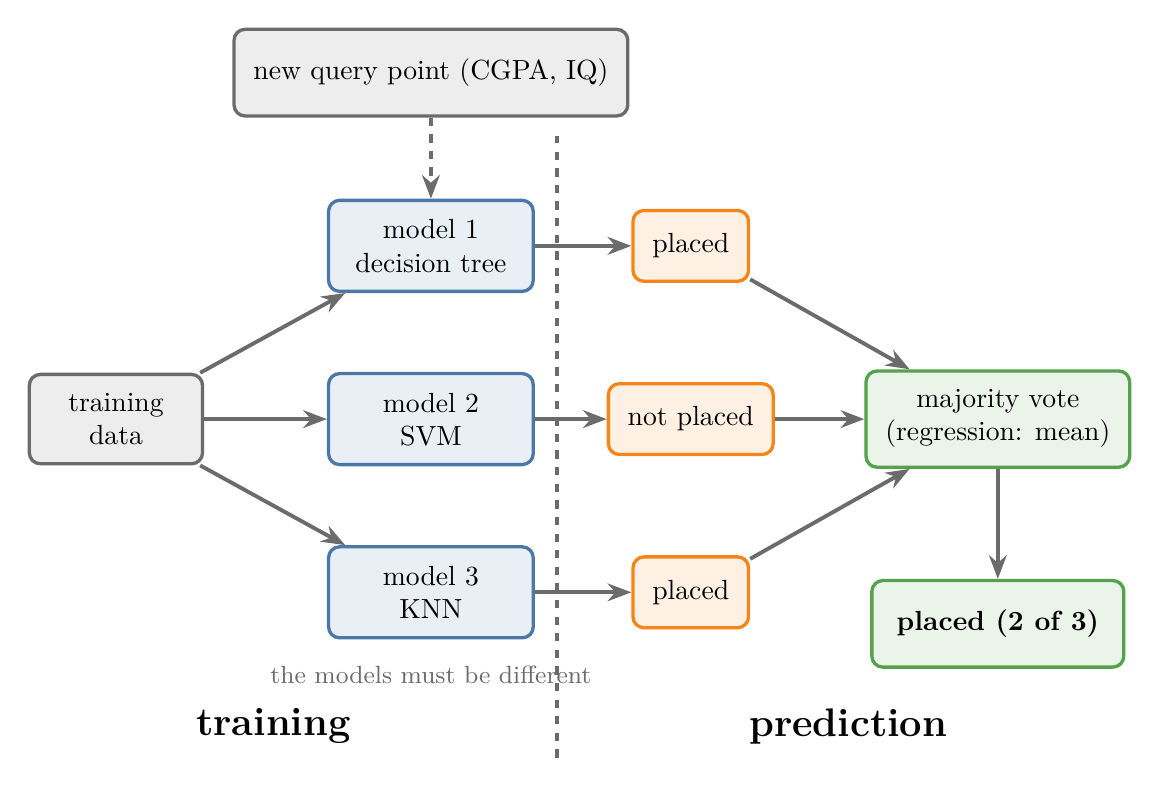
\begin{tikzpicture}[
  m/.style={box=cblue, minimum width=2.6cm},
  d/.style={box=cgrey, minimum width=2.2cm},
  p/.style={box=corange, minimum width=1.2cm, minimum height=0.9cm},
  o/.style={box=cgreen, minimum width=3.2cm}]
  % training
  \node[d] (D) at (0,0) {training\\data};
  \node[m] (m1) at (4,2.2) {model 1\\decision tree};
  \node[m] (m2) at (4,0) {model 2\\SVM};
  \node[m] (m3) at (4,-2.2) {model 3\\KNN};
  \foreach \i in {1,2,3} \draw[arrow] (D) -- (m\i);
  % prediction
  \node[d] (q) at (4,4.4) {new query point (CGPA, IQ)};
  \draw[arrow, dashed] (q) -- (m1);
  \node[p] (p1) at (7.3,2.2) {placed};
  \node[p] (p2) at (7.3,0) {not placed};
  \node[p] (p3) at (7.3,-2.2) {placed};
  \foreach \i in {1,2,3} \draw[arrow] (m\i) -- (p\i);
  \node[o] (agg) at (11.2,0) {majority vote\\(regression: mean)};
  \foreach \i in {1,2,3} \draw[arrow] (p\i) -- (agg);
  \node[o, box=cgreen, font=\sffamily\bfseries] (out) at (11.2,-2.6) {placed (2 of 3)};
  \draw[arrow] (agg) -- (out);
  \node[title] at (2,-3.9) {training};
  \node[title] at (9.3,-3.9) {prediction};
  \draw[cgrey, dashed] (5.6,-4.3) -- (5.6,3.6);
  \node[note] at (4,-3.25) {the models must be different};
\end{tikzpicture}
\end{document}
